\begin{center}
\resizebox{0.9\linewidth}{!}{%
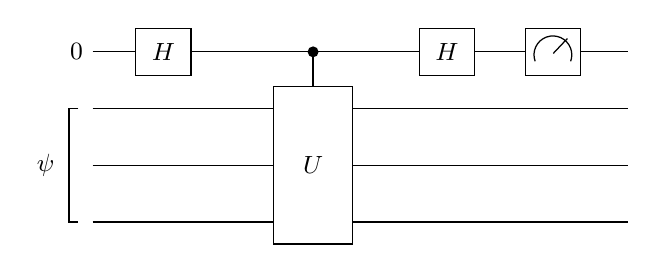
\begin{tikzpicture}[
    wire/.style={line width=0.45pt},
    gate/.style={
        draw,
        fill=white,
        minimum width=7mm,
        minimum height=6mm,
        inner sep=0pt,
        font=\small
    },
    unitary/.style={
        draw,
        fill=white,
        minimum width=10mm,
        minimum height=20mm,
        inner sep=0pt,
        font=\small
    },
    measure/.style={
        draw,
        fill=white,
        minimum width=7mm,
        minimum height=6mm,
        inner sep=0pt
    },
    control/.style={circle, fill=black, inner sep=1.4pt},
    wirelabel/.style={font=\small}
]
    \def\xstart{0}
    \def\xend{6.8}
    \foreach \y in {0,-0.72,-1.44,-2.16} {
        \draw[wire] (\xstart,\y) -- (\xend,\y);
    }

    \node[wirelabel, anchor=east] at (\xstart,0) {$\ket{0}$};
    \draw[wire] (-0.18,-0.72) -- (-0.30,-0.72) -- (-0.30,-2.16) -- (-0.18,-2.16);
    \node[wirelabel, anchor=east] at (-0.36,-1.44) {$\ket{\psi}$};

    \node[gate] at (0.9,0) {$H$};

    \node[unitary] (u) at (2.8,-1.44) {$U$};
    \draw[wire] (2.8,0) -- (u.north);
    \node[control] at (2.8,0) {};

    \node[gate] at (4.5,0) {$H$};

    \node[measure] at (5.85,0) {};
    \draw[wire] (5.62,-0.12) arc[start angle=200, end angle=-20, radius=0.24];
    \draw[wire] (5.85,-0.02) -- (6.03,0.17);
\end{tikzpicture}%
}
\end{center}
